\chapter{Ottimizzazione}
Nel corso di Machine Learning abbiamo conosciuto lo \textbf{Stochastic Gradient Descent} e alcune delle sue varianti (Batch e MiniBatch), un meccanismo attraverso il quale si cercano delle condizioni di ottimalità. In questo capitolo affronteremo proprio i problemi legati all'\textbf{Ottimizzazione} e le tecniche che hanno portato all'evoluzione e alla modifica della classica discesa del gradiente. Noi sappiamo che ogni modello è caratterizzato da parametri (pesi e bias), ed essi determinano la capacità del modello nel trasformare gli input in output. L'obbiettivo del processo di training risulta essere, trovare valori dei pesi che minimizzino l'errore. La superficie d'errore (Figura~\ref{fig:error_surface}), è spesso utilizzata per rappresentare graficamente come la funzione di costo varia al modificarsi dei pesi.

\begin{figure}[h]
    \centering
    \includegraphics[width=0.45\textwidth]{figure/error_surface.png}
    \caption{L’immagine illustra la "mappa" della funzione d’errore. Con l'errore rispetto a un peso di cui si mostra l'andamento parabolico, e il suo valore ottimizzato nel vertice (sopra). Inoltre una rappresentazione a due pesi, dove il valore ottimizzato si trova al centro delle ellissi, ognuna delle quali è una curva di livello (sotto).}
    \label{fig:error_surface}
\end{figure}

\section{Discesa del Gradiente}
La \textbf{Discesa del Gradiente} (Gradient Descent) è l’algoritmo che usiamo per muoverci sulla superficie d'errore per raggiungere il punto dove l'errore è minimo. Immaginando una pallina rotolare sulla superficie, all’inizio si trova in un punto alto (errore grande). Ad ogni passo, si muoverà nella direzione in cui la pendenza scende più rapidamente (cioè la direzione del gradiente negativo), essa continuerà a scendere fino ad arrivare in fondo alla "valle" della superficie, dove la pendenza è pari a zero (minimo locale o globale). Questa discesa si concretizza con l'aggiornamento continuo dei pesi nel seguente modo:

\[
    w_i^{(t+1)} =w_i^{(t)}-\eta\frac{\partial L}{\partial w_i}
\]

Una valutazione da effettuare di volta in volta, è con quanta velocità giungiamo alla "valle" durante la nostra discesa, questa carattiristica può variare a seconda del valore assegnato al Learning Rate ($\eta$), proprio per questo motivo, scegliere il Learning Rate diventa un fattore cruciale durante l'implementazione dell'algoritmo di discesa del gradiente.

\subsection{Scegliere il Learning Rate}
Per poter decidere il valore ottimale del Learning Rate, si inizia impostandolo ad un valore elevato, per evitare di collassare all'interno di un minimo locale troppo presto. Successivamente, attraverso tecniche di decadimento (decay), si passa a ridurlo progressivamente per aumentare la probabilità di convergenza verso un minimo globale. Tra le strategie più comuni di decadimento possiamo considerare:
\begin{itemize}
    \item\textbf{Step Decay:} il Learning Rate viene ridotto di un fattore fisso dopo un certo numero di epoche (iterazioni);
    \item\textbf{Exponential Decay:} il Learning Rate diminuisce esponenzialmente nel tempo;
    \item\textbf{Adaptive Learning Rate:} tecniche come Adam e RMSprop regolano dinamicamente, adattando il learning rate per ogni parametro della rete.
\end{itemize}

\begin{figure}[!ht]
    \centering
    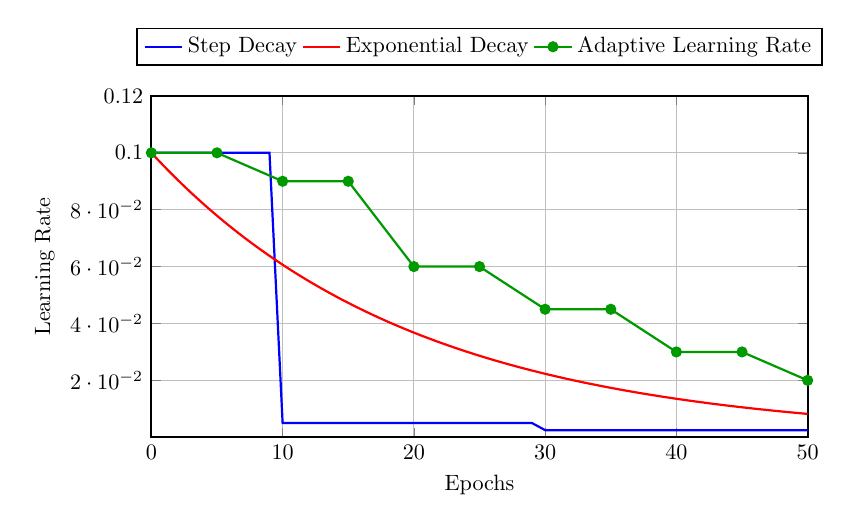
\begin{tikzpicture}[scale=0.8]
        \begin{axis}[
            width=12cm, height=7cm,
            xlabel={Epochs},
            ylabel={Learning Rate},
            xmin=0, xmax=50,
            ymin=0, ymax=0.12,
            legend style={
                at={(0.5,1.2)},
                anchor=north,
                legend columns=3
            },
            xtick={0,10,20,30,40,50},
            ytick={0.02,0.04,0.06,0.08,0.1,0.12},
            grid=both,
            thick,
            every axis plot/.append style={line width=1pt},
        ]

        \addplot[blue, domain=0:50, samples=51] 
            {0.1 * (x<10 ? 1 : (x<30 ? 0.05 : 0.025))};
        \addlegendentry{Step Decay}

        \addplot[red, domain=0:50, samples=200]
            {0.1 * exp(-0.05*x)};
        \addlegendentry{Exponential Decay}

        \addplot[green!60!black, mark=*] 
            coordinates {
                (0, 0.1) (5, 0.1) (10, 0.09) (15, 0.09)
                (20, 0.06) (25, 0.06) (30, 0.045)
                (35, 0.045) (40, 0.03) (45, 0.03) (50, 0.02)
            };
        \addlegendentry{Adaptive Learning Rate}

        \end{axis}
    \end{tikzpicture}
    \caption{Confronto tra diverse strategie di decadimento del learning rate.}
    \label{fig:lr_decay}
\end{figure}

\subsection{Inizializzazione dei pesi}
Oltre all'ottimizzazione legata al valore del Learning Rate, risulta essere cruciale inizializzare i pesi delle reti neurali in maniera opportuna. A differenza di ciò che accade in una regressione lineare in cui l'ottimizzazione è diretta, nelle reti neurali l'algoritmo di backpropagation può essere compromesso nel caso in cui i pesi della nostra rete non siano scelti accuratamente. 

\begin{Osservazione}
    Se due pesi all'interno di uno stesso layer hanno lo stesso valore iniziale, l'errore propagato all'indietro attraverso la rete, genererà gli stessi aggiornamenti, impedendo alla rete di apprendere in maniera corretta.
\end{Osservazione}

\begin{Osservazione}
    Qual'ora i pesi vengano inizializzati con valori troppo grandi, riscontreremo una possibilità di esplosione della rete neurale.
\end{Osservazione}

\begin{Osservazione}
    Se i pesi vengono inizializzati con valori troppo piccoli, potremmo incorrere in una possibile scomparsa del valore del gradiente.
\end{Osservazione}

Oltre a queste osservazioni, si potrebbe incorrere, banalmente, in una non convergenze, generando il fenomeno dell'Overshoot, in cui il gradiente oscilla in continuazione da una parte all'altra del valore minimo a cui si dovrebbe idealmente convergere.

\subsection{Xavier Glorot Initialization}
Uno dei principali metodi di Inizializzazione è quello studiato da Xavier~\cite{glorot2010understanding}, ma prima di addentrarci in esso, vediamo due definizioni fondamentali per procedere:
\begin{Definizione}[Fan-in]
    Il Fan-in è il numero di neuroni che alimentano un neurone nel layer successivo;
\end{Definizione}
\begin{Definizione}[Fan-out]
    Il Fan-out è il numero di neuroni che un dato neurone alimenta nel layer successivo;
\end{Definizione}
\begin{Esempio}
    Consideriamo un layer completamente connesso (Fully Connected, FC) con: 256 neuroni in ingresso e 512 neuroni in uscita, il suo fan-in sarà 256 e il suo fan-out sarà pari a 512.
\end{Esempio}

Tecniche come quella studiata da Xavier Glorot prendono in considerazione proprio questi aspetti, utilizzando distribuzioni gaussiane o uniformi adeguate da cui pescare i valori dei pesi, invece di pensare a un'inizializzazione casuale. L’idea chiave di questa inizializzazione conosciuta come \textbf{Xavier} è quella di scegliere i pesi in modo tale che vengano soddisfatte le due seguenti proprietà:
\begin{enumerate}
    \item La varianza dell'output di un neurone sia simile alla varianza del suo input;
    \item La varianza dei gradienti rimanga costante tra gli strati;
\end{enumerate}

In parole povere, si cerca di mantenere l'energia del segnale costante mentre attraversa la rete, sia in avanti che all'indietro. Per ottenere questo risultato, i pesi di ogni strato vengono estratti casualmente da una distribuzione (solitamente uniforme o normale) con una media nulla e una varianza specifica, nel caso della distribuzione normale, calcolata in base al numero di Fan-in e di Fan-out. Il valore della varianza solitamente è uno dei due:

\[
    \operatorname{Var}(W) = \frac{1}{n_{in}}\quad \text{o}\quad \operatorname{Var}(W)= \frac{2}{n_{in}+n_{out}}
\]

\begin{Osservazione}
    In alcuni paper scientifici la seconda formula compare con un 1 al numeratore, questa non risulta essere sbagliata in senso assoluto, ma sono due varianti della stessa idea, quella che è riportata qui si basa sul paper ufficiale~\cite{glorot2010understanding}, in cui si adotta una media armonica tra i due requisiti prendendo il nome di He Initialization, differentemente dall'altra alle volte presente, la quale adotta una media aritmetica.
\end{Osservazione}

Utilizzando una distribuzione uniforme la formula sarà la seguente:
\[
    \mathcal{U}\left(-\frac{\sqrt{6}}{\sqrt{n_{in}+n_{out}}},\,\frac{\sqrt{6}}{\sqrt{n_{in}+n_{out}}}\right)
\]

La Xavier Initialization risulta essere un miglioramento rispetto all'inizializzazione a zero o quella casuale arbitraria, perché bilancia la propagazione del segnale nei vari strati.

\subsection{Normalizzazione}
Per normalizzare i dati, possiamo utilizzare tecniche come la \textit{Min-Max Normalization} e la \textit{Z-Score Normalization}, già viste nel corso di Machine Learning, esse rendono il dataset più coerente e scalabile. Il problema di queste tecniche, però è che effettuano un'assunzione quasi mai vera, ossia che le feature risultino scorrelate fra loro. Pertanto la sfida passa ad effettuare una decorrelazione delle feature in modo efficace, risultato ottenibile in diversi modi:
\begin{enumerate}
    \item\textbf{Principal Component Analysis (PCA):} tecnica che trasforma le feature originali in nuove variabili non correlate~\cite{pearson1901pca,hotelling1933analysis};
    \item\textbf{Whitening:} trasformazione che rende le feature scorrelate con varianza unitaria~\cite{bell1995ica,hyvarinen2000ica};
    \item\textbf{Batch Normalization:} tecnica che normalizza le attivazioni durante l'addestramento per migliorare la stabilità e accelerarne la convergenza~\cite{ioffe2015batchnorm}.
\end{enumerate}

\begin{table}[!ht]
    \centering
    \caption{Confronto tra PCA, Whitening e Batch Normalization}
    \begin{adjustbox}{width=\textwidth}
    \begin{tabular}{@{} lccc @{}}
        \toprule
        \textbf{Caratteristica} & \textbf{PCA} & \textbf{Whitening} & \textbf{Batch Normalization} \\
        \midrule
        \textbf{Tipo} & Preprocessing & Preprocessing & In-training normalizzazione \\
        \textbf{Obiettivo} & Riduzione dimensionalità & Decorrelazione delle feature & Accelerare il training \\
        \textbf{Agisce su} & Intero dataset & Intero dataset & Mini-batch durante il training \\
        \textbf{Rende varianza uniforme?} & No & Sì (varianza unitaria) & No (mantiene varianza originale) \\
        \textbf{Rende feature ortogonali?} & Sì & Sì & No \\
        \textbf{Mantiene struttura dati?} & Parzialmente & Meno rispetto a PCA & Sì \\
        \textbf{Uso tipico} & Compressione dati, pretraining & Preprocessing per ICA, SVM & Normalizzazione nei layer di Reti Neurali \\
        \textbf{Effetto su reti neurali} & Riduce dimensionalità in input & Raramente usato direttamente & Migliora stabilità e velocità di training \\
        \bottomrule
    \end{tabular}
    \end{adjustbox}
\end{table}

\section{Momentum}
La Discesa del Gradiente è la base di gran parte dei metodi di ottimizzazione, nonostante la sua semplicità ed efficacia teorica, presenta alcune limitazioni pratiche. Uno dei principali problemi è la \textbf{Velocità di Convergenza} nel momento in cui la funzione di costo ha una forma fortemente non uniforme, caratterizzata da \textit{valli strette e lunghe}. In tali casi, la pendenza della funzione può risultare molto ripida in una direzione e quasi piatta in altre, di conseguenza, il vettore gradiente, non punta direttamente verso il minimo, ma tende ad alternarsi tra le direzioni di massima e minima pendenza. Il risultato è una convergenza rallentata, come se ci trovassimo fra due pareti rocciose molto ripide e man mano che scendiamo lungo un canale che è la direzione desiderata, andassimo a sbattere alle due pareti. Per mitigare tali effetti, sono stati introdotti ottimizzatori più avanzati estendendo la discesa del gradiente classica. Tra questi, primo fra tutti, il metodo del \textbf{Momentum}~\cite{polyak1964momentum} in grado di ridurre le oscillazioni, accumulando una componente inerziale nella direzione di discesa, basandosi sulla storia dei gradienti precedenti, smorzando le oscillazioni.

\begin{equation*}
    \left\{\begin{array}{c}
    v_{t} = \beta v_{t-1} - \eta\,\nabla L(w_t)
    \\
    w_{t+1} = w_t + \,v_{t}
    \end{array}\right.
\end{equation*}
\\

Con $v$ il \textit{Momentum Parameter} il quale prende in analisi la velocità di discesa fino a un determinato momento, mentre $\beta$ è il \textit{Damping Factor}, un valore che controlla quanto la velocità passata influenza quella attuale, compreso fra zero e uno. Se fosse zero, staremmo facendo semplicemente la discesa del gradiente, nel caso unitario invece avrei un'esplosione del gradiente nella nostra rete neurale. Il valore del damping factor, ci permette di capire la velocità del cambio di direzione, più sarà piccolo, più la direzione cambierà velocemente.

\begin{figure}[ht]
    \centering
    \includegraphics[width=\textwidth]{figure/DampingFactMomentum.png}
    \caption{Confronto delle traiettorie per diversi valori di $\beta$ nel Momentum.}
\end{figure}

\section{Nesterov Accelerated Gradient}
Il Momentum classico aiuta la discesa del gradiente accelerando il processo e smorzando le oscillazioni, ma ha un problema: aggiorna i pesi basandosi sulla direzione del gradiente calcolato nella posizione attuale, senza considerare dove il peso si troverà dopo l'aggiornamento. Il matematico Yurii Nesterov nel 1983 propose una modifica al Momentum classico, chiamata \textbf{Nesterov Accelerated Gradient} (NAG)~\cite{nesterov1983method,sutskever2013momentum}, migliorando la velocità di convergenza e la stabilità dell’ottimizzazione. Per comprenderne al meglio la differenza, ci basta immaginare una persona in bicicletta: nel momentum classico, la persona spinge sui pedali senza guardare avanti, e se la strada curva improvvisamente, potrei andare troppo veloce nella direzione sbagliata e dover correggere bruscamente; con il momentum di Nesterov, si guarda avanti prima di spingere sui pedali, valutando quanta forza imprimere sui pedali per correggere il movimento in base alla direzione da seguire.
\begin{figure}
    \centering
    \includegraphics[width=0.75\textwidth]{figure/momenest.png}
    \caption{Nel grafico è possibile vedere la velocità di convergenza confrontando i due Momentum entrambi partendo da uno stesso punto d'inizio, il Momentum classico come potevamo aspettarci avrà delle oscillazioni molto più grandi rispetto a quelle del Momentum di Nesterov.}
    \label{fig:MomentumVS}
\end{figure}
Il Momentum di Nesterov risulta essere più efficiente poiché calcola il gradiente in una posizione successiva vedendo in anticipo dove ci porterà la velocità calcolata, mantenendo così un'alta velocità senza instabilità.

\begin{equation*}
\left\{\begin{array}{c}
    v_{t} = \beta v_{t-1}\,-\,\eta\,\frac{\partial L}{\partial(w_t\,+\,\beta\,v_{t-1})}\\
    w_{t+1} = w_t\,+\,v_t
    \end{array}\right.
\end{equation*}

Nesterov è un piccolo ma potente miglioramento rispetto al Momentum classico. Questo metodo viene spesso usato negli ottimizzatori moderni come Adam, RMSprop con Momentum, e molte varianti di SGD, perché migliora stabilità e velocità di convergenza.

\subsection{Perché funziona il Momentum ?}
Il Momentum funziona principalmente per due motivi:
\begin{enumerate}
    \item Accelerazione dell'ottimizzazione;
    \item Attenuazione del rumore;
\end{enumerate}

\subsubsection{Accelerazione dell'ottimizzazione}
L'idea del momentum è una spinta di un carrello in discesa, se dessi un piccolo colpo, si muoverà piano, se continuo a spingere il carrello guadagnerà velocità, e qual'ora smettessi di spingere, continuerà a muoversi per inerzia. Matematicamente questo viene considerato grazie all'aggiornamento dei pesi tramite l'utilizzo di un valore che tiene conto dei valori precedenti nel calcolo del gradiente. Pertanto se i gradienti puntano nella stessa direzione per più step, la velocità aumenterà e il modello sarà portato a convergere più velocemente.
\subsubsection{Attenuazione del rumore}
Con il Momentum, accumuliamo un valore mediato nel tempo, riducendo il rumore casuale come succedeva a ogni piccola variazione. Se il rumore nei gradienti punta in direzioni casuali, questi si annullano nel tempo, il movimento risulta più fluido e meno oscillante e infine permette di superare piccoli ostacoli senza rimanere bloccati in minimi locali poco profondi. Il Momentum di Nesterov, migliora ulteriormente entrambi gli aspetti anticipando il passo successivo prima di aggiornare la velocità, evitando così di andare troppo oltre e migliorando la precisione.

\section{Learning Rate adattivo}
I parametri presenti in un modello, possono avere delle tipologie di scale di aggioranmento differenti, proprio per questo nasce l'idea di creare un \textbf{Learning Rate adattivo}. Prendendo una direzione di discesa al posto di un'altra, potremmo ritrovarci con richieste di un learning rate più grande o più piccolo, se ne usassimo uno fisso per tutti i parametri porterebbero a delle oscillazioni, o convergenze dilatate nel tempo. Quindi viene deciso di adattare il learning rate in modo indipendente per ogni parametro, basandosi sull'andamento del gradiente.

\subsection{Additive increase multiplicative decrease}
Adattare il learning rate individualmente per ogni peso con un piccolo incremento e un decremento moltiplicativo nasce per poter bilanciare due aspetti:
\begin{itemize}
    \item Gradiente coerente in una direzione $\rightarrow$ Aumentiamo il Learning Rate accelerando la convergenza;
    \item Gradiente cambia direzione frequentemente $\rightarrow$ Riduciamo il Learning Rate evitando oscillazioni.
\end{itemize}

Questa tecnica è utilizzata in metodi come \textbf{Adadelta}, \textbf{Rprop} (Resilient Propagation) e alcune varianti di \textbf{Adam}, tutte tecniche che vedremo a breve. Il funzionamento è semplice: nel momento in cui valuto i singoli Learning Rate, se il gradiente mantiene la stessa direzione, aumento il valore del Learning Rate per fare passi più grandi, diversamente se cambia di segno, significa che stiamo oscillando troppo, perciò lo ridurremo per stabilizzarlo.

\section{Resilient Propagation (Rprop)}

La \textbf{Resilient Propagation} (Rprop), introdotta da Riedmiller et al. 1993~\cite{RiedmillerBraun1993}, è un metodo di ottimizzazione che affronta una delle principali debolezze della discesa del gradiente: la dipendenza dalla magnitudine. L'idea consiste nel considerare unicamente il \textit{segno} del gradiente per determinare la direzione di aggiornamento, mentre la grandezza del passo di apprendimento viene adattata dinamicamente per ciascun peso in modo indipendente. Per ogni parametro $w_i$ si definisce un valore di aggiornamento $\Delta_i(t)$, regolato in base alla coerenza del segno del gradiente nel tempo:
\[
    \Delta_i(t) =
    \begin{cases}
        \eta^+ \cdot \Delta_i(t-1), & \text{se } \frac{\partial L(t-1)}{\partial w_i} \cdot \frac{\partial L(t)}{\partial w_i} > 0 \\[6pt]
        \eta^- \cdot \Delta_i(t-1), & \text{se } \frac{\partial L(t-1)}{\partial w_i} \cdot \frac{\partial L(t)}{\partial w_i} < 0 \\[6pt]
        \Delta_i(t-1), & \text{altrimenti}
    \end{cases}
\]
Solitamente $\eta^+$ e $\eta^-$ hanno un valore rispettivamente di $1.2$ e $0.5$, l'aggiornamento del peso avviene quindi come:
\[
    w_i(t+1) = w_i(t) - \operatorname{sign}\!\left(\frac{\partial L(t)}{\partial w_i}\right) \cdot \Delta_i(t)
\]

In questo modo, ciascun peso dispone di un proprio Learning Rate, che cresce quando la direzione del gradiente è coerente, e diminuisce quando essa si inverte. Tale meccanismo permette di accelerare la convergenza nelle regioni piatte della funzione di costo e di ridurre le oscillazioni nelle zone di forte curvatura.

\section{RMSprop}

Dopo gli approcci basati su aggiornamenti indipendenti dei pesi, come la \textbf{Resilient Propagation}, la ricerca sull’ottimizzazione dei modelli neurali si è orientata verso metodi in grado di adattare dinamicamente il Learning Rate in base al comportamento locale del gradiente. Uno dei risultati più efficaci in questa direzione è l’algoritmo \textbf{RMSprop} (\textit{Root Mean Square Propagation}), introdotto da Geoffrey Hinton nel 2012~\cite{TielemanHinton2012RMSprop}. Stabilizzando la discesa del gradiente tramite il passo di aggiornamento di ciascun parametro, in funzione della sua storia recente di variazioni. Per evitare questo problema, RMSprop introduce una \textit{media mobile esponenziale} dei quadrati dei gradienti, per mantenere un bilanciamento costante tra memoria storica e reattività alle variazioni recenti. Formalmente, il valore medio viene aggiornato secondo:
\[
    E[g^2]_t = \gamma E[g^2]_{t-1} + (1 - \gamma) (\nabla L(w_t))^2
\]
dove $\gamma$ rappresenta il fattore di decadimento (tipicamente pari a 0.9) e $\nabla L(w_t)$ è il gradiente calcolato al passo $t$. L’aggiornamento dei pesi diventa quindi:
\[
    w_{t+1} = w_t - \frac{\eta}{\sqrt{E[g^2]_t + \epsilon}} \, \nabla L(w_t)
\]
dove $\eta$ è il learning rate ed $\epsilon$ una piccola costante per evitare divisioni per zero. In questo modo, ciascun parametro dispone di un proprio passo di apprendimento adattivo:  
\begin{itemize}
    \item Se un peso riceve gradienti di grande ampiezza, il termine $E[g^2]_t$ cresce e il passo verrà ridotto, prevenendo oscillazioni e instabilità;
    \item Se i gradienti risultano piccoli o irregolari, il passo resterà più ampio, accelerando la convergenza.
\end{itemize}

RMSprop si distingue quindi come una strategia di ottimizzazione \textit{localmente adattiva}, capace di bilanciare velocità e stabilità. Essa rappresenta il punto di transizione naturale tra i metodi a passo variabile per singolo parametro, come Rprop, e le tecniche completamente adattive di generazione successiva, come \textbf{AdaGrad}, che approfondiremo nella sezione seguente.


\section{AdaGrad}

L’algoritmo \textbf{AdaGrad} (\textit{Adaptive Gradient}) rappresenta uno dei primi approcci di ottimizzazione realmente \textit{adattivi}, introdotto da Duchi et al. 2011~\cite{DuchiHazanSinger2011AdaGrad}. La sua idea di fondo è quella di modificare dinamicamente il tasso di aggiornamento per ciascun parametro del modello, in modo da rendere l’aggiornamento più sensibile alla frequenza e all’intensità dei gradienti associati a ogni peso. Nella discesa del gradiente tradizionale, un singolo valore di \textit{Learning Rate} $\eta$ viene applicato uniformemente a tutti i pesi. Ma i diversi parametri di una rete neurale possono contribuire in misura molto diversa alla funzione di costo: alcuni ricevono gradienti ampi e frequenti, altri piccoli o sporadici. AdaGrad affronta questo problema regolando automaticamente l’ampiezza del passo per ciascun peso in modo inversamente proporzionale alla somma cumulativa dei suoi gradienti al quadrato. Formalmente, si definisce per ogni parametro $w_i$ un accumulatore $G_i(t)$:
\[
    G_i(t) = \sum_{k=1}^{t} \left( \frac{\partial L(w_i^{(k)})}{\partial w_i} \right)^2
\]
e l’aggiornamento dei pesi avviene come:
\[
    w_i^{(t+1)} = w_i^{(t)} - \frac{\eta}{\sqrt{G_i(t) + \epsilon}} \, \frac{\partial L(w_i^{(t)})}{\partial w_i}
\]
dove $\epsilon$ è una piccola costante di stabilità numerica. Parametri che ricevono gradienti grandi in modo persistente avranno un denominatore elevato, quindi un passo di aggiornamento più piccolo; viceversa, quelli con gradienti rari o deboli verranno aggiornati con passi più ampi. Il risultato è un'\textbf{auto-regolazione locale del learning rate} che porta al miglioramento della convergenza. La caratteristica di AdaGrad di accumulare indefinitamente il quadrato dei gradienti comporta un effetto collaterale significativo: con il progredire dell’addestramento, $G_i(t)$ cresce costantemente, facendo diminuire il Learning Rate fino a valori prossimi allo zero. Portando a un \textbf{prematuro rallentamento della convergenza}, specialmente nelle fasi finali dell’ottimizzazione, quando il modello necessiterebbe ancora di piccoli aggiustamenti. Per ovviare a questo problema, sono state introdotte varianti più flessibili, come \textbf{Adadelta}, in grado di mantenere l’adattività di AdaGrad ma sostituendo la somma cumulativa, con una media mobile esponenziale dei gradienti al quadrato, preservando così un equilibrio più stabile nel tempo.

\section{Adadelta}

L’algoritmo \textbf{Adadelta}, proposto da Zeiler nel 2012~\cite{Zeiler2012AdaDelta}, nasce come evoluzione di \textbf{AdaGrad}, con l’obiettivo di risolvere il problema del decadimento eccessivo del Learning Rate dovuto all’accumulo dei gradienti al quadrato. Come visto nella sezione precedente, AdaGrad ostacola la capacità del modello di continuare ad apprendere nelle fasi avanzate dell’addestramento. L’idea di Adadelta è sostituire la somma cumulativa con una \textbf{media mobile esponenziale} dei gradienti al quadrato, mantenendo una memoria a breve termine della loro variazione. In questo modo, l’algoritmo conserva la natura adattiva di AdaGrad, ma elimina il rallentamento asintotico. Formalmente, per ciascun parametro $w_i$, la media mobile viene aggiornata secondo:
\[
    E[g_i^2]_t = \rho E[g_i^2]_{t-1} + (1 - \rho) \left( \frac{\partial L(w_i^{(t)})}{\partial w_i} \right)^2
\]
dove $\rho$ è il fattore di decadimento esponenziale (tipicamente compreso tra 0.9 e 0.95). L’ampiezza del passo viene poi calcolata come:
\[
    \Delta w_i^{(t)} = - \frac{\sqrt{E[\Delta w_i^2]_{t-1} + \epsilon}}{\sqrt{E[g_i^2]_t + \epsilon}} \, \frac{\partial L(w_i^{(t)})}{\partial w_i}
\]
e infine i pesi vengono aggiornati come segue:
\[
    w_i^{(t+1)} = w_i^{(t)} + \Delta w_i^{(t)}
\]

Un aspetto distintivo di Adadelta è l’introduzione di una seconda media mobile $E[\Delta w_i^2]_t$, tenente traccia dell’ampiezza media degli aggiornamenti precedenti. Questo termine funge da \textbf{meccanismo di autoregolazione del passo}, consentendo all’algoritmo di adattare dinamicamente non solo la direzione, ma anche la scala delle variazioni dei pesi. Il risultato è un comportamento più stabile e coerente, che non richiede l’impostazione manuale di un learning rate globale. Grazie a queste caratteristiche, Adadelta è particolarmente efficace in scenari in cui i gradienti variano in modo non uniforme o decrescono rapidamente nel tempo. Il metodo può essere interpretato come un ponte concettuale tra AdaGrad e gli ottimizzatori successivi, i quali ereditano il principio di adattività locale combinandolo con strategie di momentum e media mobile dei gradienti. In sintesi, Adadelta introduce una forma di apprendimento adattivo completamente autonoma, in grado di bilanciare efficacemente velocità di convergenza e stabilità numerica senza dipendere da un Learning Rate fisso.

\section{Adam}

L’algoritmo \textbf{Adam} (\textit{Adaptive Moment Estimation}), proposto da Kingma et al. 2015~\cite{KingmaBa2015Adam}, rappresenta una delle più efficaci e diffuse tecniche di ottimizzazione nel Deep Learning moderno. Adam combina i principi del \textbf{momentum} e dei metodi \textbf{adattivi} come \textbf{RMSprop}, fornendo un aggiornamento dei pesi: stabile, veloce e robusto rispetto alle variazioni della scala dei gradienti. L’idea consiste nel mantenere due medie mobili esponenziali:
\begin{itemize}
    \item Una per la \textbf{stima del primo momento} (la media dei gradienti), analoga al momentum classico;
    \item Una per la \textbf{stima del secondo momento} (la media dei quadrati dei gradienti), come in RMSprop.
\end{itemize}

Formalmente, per ciascun parametro $w_i$, al passo $t$ si definiscono:
\[
    m_t = \beta_1 m_{t-1} + (1 - \beta_1) \nabla L(w_t)
\]
\[
    v_t = \beta_2 v_{t-1} + (1 - \beta_2) (\nabla L(w_t))^2
\]
dove:
\begin{itemize}
    \item $m_t$ rappresenta la stima del primo momento (velocità media),
    \item $v_t$ rappresenta la stima del secondo momento (varianza),
    \item $\beta_1$ e $\beta_2$ sono coefficienti di decadimento esponenziale, tipicamente $\beta_1 = 0.9$ e $\beta_2 = 0.999$.
\end{itemize}

Entrambe le stime vengono inizializzate a zero al primo passo, proprio per questo Adam applica una correzione al bias introdotto dalle prime iterazioni trasformando le stime dei due momenti come segue:
\[
    \hat{m}_t = \frac{m_t}{1 - \beta_1^t}, \qquad
    \hat{v}_t = \frac{v_t}{1 - \beta_2^t}
\]
Una volta calcolate le stime dei due momenti, si passa all'aggiornamento dei pesi:
\[
    w_{t+1} = w_t - \frac{\eta}{\sqrt{\hat{v}_t} + \epsilon} \, \hat{m}_t
\]
dove $\eta$ rappresenta il Learning Rate, mentre $\epsilon$ una costante di stabilità numerica (solitamente $10^{-8}$). Grazie a questa formulazione, Adam unisce:
\begin{itemize}
    \item\textbf{Stabilità} dei metodi basati su media mobile (come RMSprop), che riducono il passo nelle direzioni ad alta curvatura;
    \item\textbf{Velocità di convergenza} del momentum, che mantiene la direzione media di discesa evitando oscillazioni.
\end{itemize}

L’algoritmo si adatta automaticamente alla scala dei gradienti di ciascun parametro, eliminando la necessità di un fine tuning del Learning Rate e rendendolo particolarmente efficace in reti profonde o con dati rumorosi. Per questo motivo, Adam è oggi uno degli ottimizzatori di default in numerosi framework di Deep Learning e architetture moderne (Transformer, GAN, reti convoluzionali, ecc.).

\subsection{Limitazioni di Adam}
Adam non risulta essere perfetto, poiché incorre in alcune limitazioni:
\begin{itemize}
    \item\textbf{Sovra-adattamento ai dati rumorosi:} Adam si adatta velocemente, ma può adattarsi troppo a gradienti rumorosi, riducendo la capacità del modello di generalizzazione;
    \item \textbf{Decay inefficace del peso:} Adam non fa un vero weight decay come la discesa del gradiente classica. Nel SGD viene incluso il parametro di regolarizzazione, in Adam viene fatta tramite il learning rate adattivo, dunque risulta essere meno efficace;
    \item\textbf{Rallentata convergenza finale:} Adam spesso converge rapidamente all'inizio, ma poi rallenta molto nel trovare il minimo ottimale. Questo poiché i Learning Rate adattivi riducono troppo la velocità di aggiornamento nelle fasi finali.
\end{itemize}
Proprio per cercare di mitigare questi comportamenti, è stata introdotta una variante evoluta di Adam, più stabile, la quale prende il nome di \textbf{AdamW}.
\begin{figure}
    \centering
    \includegraphics[width=0.7\textwidth]{figure/sgrmspropadam.png}
    \caption{Grafico che mette in luce le differenze nella convergenza fra lo SGD, la RMSprop e Adam}
    \label{fig:diffAdamSGDRMSprop}
\end{figure}

\subsection{AdamW}

L’ottimizzatore \textbf{AdamW} (\textit{Adam with Weight Decay}), proposto da Loshchilov et al. 2017~\cite{LoshchilovHutter2017AdamW}, modifica la regolarizzazione di Adam separando esplicitamente il termine di \textit{weight decay} dall’aggiornamento del gradiente. Nel metodo Adam classico, la penalizzazione $L_2$ sui pesi viene incorporata nel gradiente stesso, alterando le medie mobili e introducendo interazioni indesiderate con il meccanismo adattivo. AdamW rimuove questa interferenza applicando il decadimento dei pesi come un’operazione separata:
\[
    w_{t+1} = w_t - \eta \lambda w_t - \frac{\eta}{\sqrt{\hat{v}_t} + \epsilon} \, \hat{m}_t
\]
dove $\lambda$ è il coefficiente di \textit{weight decay}. Questa semplice modifica migliora la \textbf{generalizzazione} e la \textbf{stabilità numerica}, specialmente nei contesti di addestramento di grandi modelli come BERT e GPT. AdamW è oggi la variante di riferimento dell’ottimizzatore Adam ed è implementato come impostazione predefinita nei principali framework di Deep Learning.

\section{Lion}
Adam è l'ottimizzatore più utilizzato nel campo della ricerca, ma nonostante ciò, non risulta essere il migliore, nel Febbraio del 2023, è stato proposto un ottimizzatore completamente diverso da quelli precedenti, perché proposto da un Agente di Intelligenza Artificiale. Crearlo tramite un calcolatore, ha portato a raffinare le formule trasponendole direttamente in linee di codice, dando la possibilità di considerarne l'impatto sul costo computazionale. Per rendere più compatto il codice, l'agente ha introdotto una funzione, che è esattamente quella presente in tutti gli ottimizzatori che abbiamo visto fin'ora (funzione di interpolazione). L'algoritmo utilizzato per trovare Lion permetteva di analizzare vari ottimizzatori, migliorati nei vari cicli di aggiornamento, effettuando di volta in volta un torneo fra loro, in modo da combinarne i migliori e generarne dei figli adottando i pregi dei genitori, permettendo di raffinarsi sempre più, esattamente come accade con le manipolazioni genetiche. Di seguito il codice implementativo di Lion:

\begin{python}[frame=trBL] 
    def train(weight, gradient, momentum, lr): 
        update = interp(gradient, momentum, (*@$\beta_1$@*)) 
        update = sign(update) 
        momentum = interp(gradient, momentum, (*@$\beta_2$@*))
        weight_decay = weight * (*@$\lambda$@*) 
        update = update + weight_decay 
        update = update * lr 
    return update, momentum 
\end{python}

\section{Gradiente e Curvatura}
Scegliendo la direzione in cui convergere, è corretto chiedersi di quanto diminuisca l'errore prima di ricomonciare a salire, solitamente, si assume la curvatura costante, cioè una superficie di errore quadratica, assumiamo nella nostra analisi che l'entità del gradiente diminuisca man mano che ci spostiamo verso il basso. La riduzione massima dell'errore dipende dal rapporto fra il gradiente e la curvatura, e una buona direzione nella quale è efficiente muoversi è quella con un elevato rapporto fra gradiente e curvatura, dunque escludere la derivata seconda in ogni direzione, è un'approssimazione, considerarla, ci permette di aumentare la generalizzazione dei nostri algoritmi di convergenza, pertanto il giusto interrogativo da porsi risulta essere come trovare il giusto valore del rapporto.

\section{Metodo di Newton}
Il \textbf{Metodo di Newton}~\cite{NocedalWright2006NumericalOptimization} è la soluziona a questo interrogativo, integrando la curvatura e il gradiente, moltiplicando la matrice Hessiana con il gradiente stesso. Prima di entrare nel fulcro del metodo di Newton, ricordiamo un paio di concetti fondamentali.

\subsubsection{Gradiente}
Sia $f:\mathbb{R}^n \rightarrow \mathbb{R}$ un campo scalare. Il gradiente $\nabla f:\mathbb{R}^n \rightarrow \mathbb{R}^n$ è un vettore tale che $(\nabla f)_i = \frac{\partial f}{\partial x_i}$. Poiché ogni punto nel dominio di $f$ è mappato in un vettore, allora $\nabla f$ è uno spazio vettoriale.

\subsubsection{Jacobian}
Sia $\mathbf{F}:\mathbb{R}^n \rightarrow \mathbb{R}^m$ un campo vettoriale. Allora il Jacobiano può essere considerato come il campo vettoriale delle derivate. Considerando ogni componente di $\mathbf{F}$ come una singola funzione, il Jacobiano pertanto è una matrice la quale i-esima riga è il gradiente dell'i-esima componente di $\mathbf{F}$, dunque se il Jacobiano è $J$ allora:
\[
    J_{i,j} = \frac{\partial F_i}{\partial x_j}
\]

\subsubsection{Hessiano}
L'Hessiano è la matrice delle derivate seconde parziali di ogni combinazione di elementi:
\[
    H_{ij} = \frac{\partial^2 J}{\partial x_i \partial x_j}
\]
\begin{itemize}
    \item Le \textbf{componenti diagonali} indicano la curvatura lungo un singolo asse, coincidendo con la derivata seconda;
    \item Gli \textbf{elementi fuori diagonale} descrivono le interazioni tra i pesi.
\end{itemize}
Ogni elemento della matrice Hessiana, specifica come il gradiente si modifica in una direzione, nel momento in cui ci muoviamo in un'altra direzione diversa da quella del gradiente. Il metodo di Newton introduce tramite l'utilizzo dell'inversione della matrice Hessiana la seguente relazione:

\[
    \Delta w = -\epsilon H(w)^{-1}\frac{d L}{d w}
\]

Aggiungendo un'informazione non solo sul primo ordine, come avviene con i gradienti, ma anche sul secondo ordine, avendo una: precisione maggiore e una velocità di convergenza migliore. Tuttavia questo risulta essere problematico, poiché calcolare una matrice inversa, oltre ad essere computazionalmente elevato, non sempre risulta essere possibile.

\begin{Osservazione}
    L'intuizione di utilizzare l'Hessiana risiede dal fatto che il gradiente ci fornisce l'informazione della direzione in cui muoverci, mentre l'Hessiana dice di quanto curvare il passo. La discesa del gradiente segue la pendenza più ripida, Newton invece "raddrizza" la traiettoria tenendo conto della curvatura.
\end{Osservazione}

\subsection{Metodi alternativi per gestire l'Hessiano}

Calcolare l'inverso della matrice Hessiana \( H \) è computazionalmente complesso (\(O(n^3)\)) e spesso impraticabile per modelli di grandi dimensioni. Per questo motivo sono stati sviluppati diversi per ovviare a questa difficoltà, a partire dai Metodi quasi-Newton, i quali effettuano una stima di \(H\) basandosi sulle informazioni dei gradienti precedenti, o \textbf{Metodi Hessian-Free} come quello del \textit{metodo del gradiente coniugato} per minimizzare l'errore di ottimizzazione. Recentemente, questa famiglia di tecniche è stata estesa anche a contesti più complessi, come l'\textit{Online Certified Unlearning}, in cui si richiede di rimuovere selettivamente l’influenza di specifici dati di addestramento senza dover riaddestrare completamente il modello. Un esempio significativo è il lavoro di~\textcite{Qiao2023HessianFreeUnlearning}, che propone un approccio \textbf{Hessian-Free Online Certified Unlearning}, nel quale l’informazione di secondo ordine viene stimata in modo efficiente per garantire una rimozione certificata e stabile dei dati. Tale metodologia dimostra come i principi dei metodi Hessian-Free possano essere estesi anche a problemi di sicurezza e robustezza dei modelli di apprendimento automatico.

\section{Gradiente Coniugato}

Il \textbf{Metodo del Gradiente Coniugato} rappresenta un'alternativa efficiente al metodo di Newton per la ricerca del minimo di una funzione di costo, in quanto consente di evitare l'inversione esplicita della matrice Hessiana. Il metodo del Gradiente Coniugato, evolve quello del Gradiente Classico, effettuando una serie di step affinché si trovi il minimo in una direzione, una volta ottenuto, procedo lungo un'altra direzione lasciando intatto il minimo lungo la direzione precedente (gradiente), trovando quello della direzione attuale. Se soddisfano questa caratteristica, le direzioni sono dette \textbf{coniugate} fra loro, da cui deriva il nome del metodo, il quale si articola nel seguente modo:
\begin{enumerate}
    \item Si sceglie una direzione iniziale proporzionale al gradiente: 
    \[
        d_0 = -\nabla L(w_0);
    \]
    \item Si determina il passo ottimale lungo tale direzione:
    \[
        \alpha_0 = \arg\min_{\alpha}\, L(w_0 + \alpha\, d_0);
    \]
    \item Si effettua l'aggiornamento del peso:
    \[
        w_{1} = w_0 + \alpha_0\, d_0;
    \]
    \item Si calcola una nuova direzione che sia \textbf{coniugata} rispetto all'Hessiana, ossia ortogonale rispetto alla metrica indotta da \( H \):
    \[
        d_{1} = -\nabla L(w_{1}) + \beta_1 d_1
    \]
    dove il coefficiente $\beta$ può essere calcolato come:
    \[
        \beta_1 = \frac{\nabla L(w_{1})^T \nabla L(w_{1})}{\nabla L(w_0)^T \nabla L(w_0)}.
    \]
\end{enumerate}

Ovviamente questa procedura è iterativa, pertanto basta sostituire i pedici, con il passo corretto a cui sto iterando,
la grandezza di questo metodo risiede nella posibilità di al più \( N \) iterazioni in uno spazio di dimensione \( N \), il gradiente coniugato raggiunge il minimo esatto per una funzione quadratica, evitando oscillazioni e migliorando sensibilmente la velocità di convergenza rispetto alla discesa del gradiente standard.
